\documentclass[11pt]{article}

% rlatex: compiler: 'latexmk -pdf'
% rlatex: output: pdf
% rlatex: include: sin(x).png

%Packets for graphs
\usepackage{graphicx}
\usepackage{epstopdf}
%Boxed figures
\usepackage{float}
\floatstyle{boxed} 
\restylefloat{figure}

\author{John Doe} \title{Sample Document}
\begin{document}
\maketitle

\section{Introduction}

According to the handbook of van Leunen \cite{vanleunen},
this paragraph---and certainly this
section---should be longer than one sentence.

\section{Sine}

In mathematics, the sine function is a function of an angle. In a right triangle, 
sine gives the ratio of the length of the side opposite to an angle to the length 
of the hypotenuse.

\begin{figure}[h]
    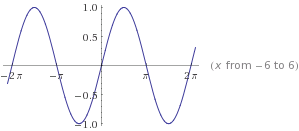
\includegraphics{sin(x).png}
    \caption{Sample $\sin(x)$ graph}
\end{figure}

Sine is usually listed first amongst the trigonometric functions.

Trigonometric functions are commonly defined as ratios of two sides of a right 
triangle containing the angle, and can equivalently be defined as the lengths of 
various line segments from a unit circle. More modern definitions express them as 
infinite series or as solutions of certain differential equations, allowing their 
extension to arbitrary positive and negative values and even to complex numbers.

The sine function is commonly used to model periodic phenomena such as sound and 
light waves, the position and velocity of harmonic oscillators, sunlight intensity
and day length, and average temperature variations throughout the year.

The function sine can be traced to the jyā and koṭi-jyā functions used in Gupta 
period Indian astronomy (Aryabhatiya, Surya Siddhanta), via translation from Sanskrit 
to Arabic and then from Arabic to Latin.[1] The word "sine" comes from a Latin 
mistranslation of the Arabic jiba, which is a transliteration of the Sanskrit 
word for half the chord, jya-ardha.

\section{More references}

Here we see if the reference \cite{Narendra_1990}
to the Narendra article comes out OK, in particular,
with volume, number \& pages.

The necessary information for those who would use BibTeX
is available in the 1988 document of Prof.\ Patashnik \cite{btxdoc}.
Interested readers who can read French may also
want to read Poussin's proof\cite{primes}, though
it has nothing at all to do with BibTeX.

\section{Conclusion}

This is the concluding paragraph.  Here I cite another of
Oren Patashnik's books\cite{btxhak} and, again,
van Leunen's and Poussin's \cite{vanleunen,primes}.

\bibliographystyle{plain}	% (uses file "plain.bst")
\bibliography{myrefs}		% expects file "myrefs.bib"
\end{document}
